
\de{ĐỀ THI HỌC KỲ I NĂM HỌC 2022-2023}{THPT Nguyễn Công Trứ}



\begin{bt}%[0T2Y2-1]%[Dự án đề kiểm tra HK1 NH22-23-Don Lee]%[THPT Nguyễn Công Trứ]
	Hãy liệt kê $2$ nghiệm của hệ bất phương trình $\heva{&x \geq 2\\&2 x+y-8 \leq 0.}$
	\loigiai{
		Ta có $(2;4)$, $(2;3)$ là nghiệm của hệ phương trình.
	}
\end{bt} 

\begin{bt}%[0T3Y1-1]
	Tìm tập xác định của hàm số $y=\dfrac{2}{\sqrt{x-2}}$.
	\loigiai{
		Điều kiện xác định $x-2>0 \Leftrightarrow x>2$.\\
		Tập xác định của hàm số $\mathscr{D}=(2;+\infty)$.
	}
\end{bt} 

\begin{bt}%[0T5B4-1]%[Dự án đề kiểm tra HK1 NH22-23-Don Lee]%[THPT Nguyễn Công Trứ]
	Cho tam giác $ABC$ đều cạnh $a$. Tính $\overrightarrow{AB} \cdot \overrightarrow{BC}$.
	\loigiai{
		Ta có $\overrightarrow{AB} \cdot \overrightarrow{BC}=\left|\overrightarrow{AB}\right|\cdot\left|\overrightarrow{BC}\right|\cdot\cos\left(\overrightarrow{AB}, \overrightarrow{BC}\right)=a\cdot a\cdot \cos 120^\circ=-\dfrac{1}{2}a^2$.
	}
\end{bt} 

\begin{bt}%[0T6Y1-2]%[Dự án đề kiểm tra HK1 NH22-23-Don Lee]%[THPT Nguyễn Công Trứ]
	Quy tròn số $\bar{a}=\sqrt{5}=2{,}236067977 \ldots$ với độ chính xác đến hàng phần trăm.
	\loigiai{
		Quy tròn số $\bar{a}=\sqrt{5}=2{,}236067977 \ldots$ với độ chính xác đến hàng phần trăm ta được $\bar{a}=\sqrt{5}=2{,}24$.
	}
\end{bt} 

\begin{bt}%[0T1B2-3]%[Dự án đề kiểm tra HK1 NH22-23-Don Lee]%[THPT Nguyễn Công Trứ]
	Cho hai tâp hợp $A=[-3; 4]$ và $B=(-\infty; 1)$. Tìm $A \cap B$, $A \cup B$, $B \setminus A$, $C_{\mathbb{R}} A$.
	\loigiai{
			Ta có 
		\begin{itemize}
		\item $A \cap B=[-3; 1)$;
		\item $A \cup B=(-\infty; 4]$;
		\item $B \backslash A=(-\infty;-3)$;
		\item $C_{\mathbb{R}} A=(-\infty;-3) \cup(4;+\infty)$.
		\end{itemize}
	}
\end{bt} 


\begin{bt}%[0T4Y2-1]%[Dự án đề kiểm tra HKI NH22-23-Trương Đăng Khoa]%[THPT Nguyễn Công Trứ]
	Cho tam giác $A B C$ có $\widehat{B}=60^{\circ}$, $\widehat{C}=45^{\circ}$ và $AB=5$. Tính độ dài cạnh $AC$ (qui tròn kết quả đến hàng phần trăm).
	\loigiai{
		Áp dụng định lí hàm số $\sin$ vào tam giác $ABC$ ta có
		\begin{eqnarray*}
			&&\dfrac{AB}{\sin \widehat{C}}=\dfrac{AC}{\sin \widehat{B}}\\
			&\Rightarrow& \dfrac{5}{\sin 45^\circ}=\dfrac{AC}{\sin 60^\circ}\\
			&\Leftrightarrow& AC =\dfrac{5\cdot \sin 60^\circ}{\sin 45^\circ}\\
			&\Leftrightarrow& AC=\dfrac{5\sqrt{6}}{2}\approx 6{,}12.
		\end{eqnarray*}
		Vậy $AC\approx 6{,}12$.
	}
\end{bt} 



\begin{bt}%[0T6Y1-2]%[Dự án đề kiểm tra HKI NH22-23-Trương Đăng Khoa]%[THPT Nguyễn Công Trứ]
	Quy tròn số $\bar{a}=7216{,}4$ đến hàng đơn vị, ta được số gần đúng $a=7216$. Tìm sai số tuyệt đối $\Delta_a$ và sai số tương đối $\delta_a$ của số gần đúng $a$.
	\loigiai{
		\begin{itemize}
			\item Sai số tuyệt đối
			$\Delta_a=\left| 7216{,}4-7216\right|=0{,}4$.
			\item Sai số tương đối 
			$\delta_a=\dfrac{\Delta_a}{|a|}=\dfrac{0{,}4}{7216}=\dfrac{1}{18040}$.
		\end{itemize}
	}
\end{bt} 



\begin{bt}%[0T3K2-2]%[Dự án đề kiểm tra HKI NH22-23-Trương Đăng Khoa]%[THPT Nguyễn Công Trứ]
	\immini{
		Cho parabol $(P)\colon y=a x^2+b x+c$, ($a \neq 0$) như hình vẽ. Xác định các hệ số $a$, $b$, $c$ của $(P)\colon y=a x^2+b x+c$, ($a \neq 0$).
	}{
		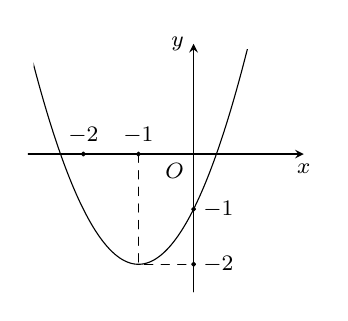
\begin{tikzpicture}[scale=0.7,>=stealth, font=\footnotesize, line join=round, line cap=round]
			\def\a{1} \def\b{2} \def\c{-1} % Hệ số
			\def\xmin{-3} \def\xmax{2}
			\def\ymin{-2.5} \def\ymax{2} 
			%	\draw[color=gray!50,dashed] (\xmin,\ymin) grid (\xmax,\ymax); 
			\draw[->] (\xmin,0)--(\xmax,0) node [below]{$x$};
			\draw[->] (0,\ymin)--(0,\ymax) node [left]{$y$};
			\node at (0,0) [below left]{$O$};
			\clip (\xmin+0.1,\ymin+0.1) rectangle (\xmax-0.5,\ymax-0.1);
			\draw[smooth,samples=300] plot(\x,{\a*(\x)^2+\b*(\x)+\c});
			\draw[dashed] (-1,0)|-(0,-2);
			\draw[fill=black]
			(-1,0)node[above]{$-1$}circle(1pt)
			(-2,0)node[above]{$-2$}circle(1pt)
			(0,-1)node[right]{$-1$}circle(1pt)
			(0,-2)node[right]{$-2$}circle(1pt);
		\end{tikzpicture}
	}
	\loigiai{Đặt $A(0;-1)$, $B(-1;-2)$.\\
		Ta có 
		$\heva{&A(0;-1)\in (P)\colon y=ax^2+bx+c\\ &B(-1;-2)\in (P)\colon y=ax^2+bx+c}\Leftrightarrow \heva{&-1=a\cdot 0^2+b\cdot 0+c\\ & -2=a\cdot (-1)^2+b \cdot (-1)+c}\Leftrightarrow \heva{& c=-1\\ &a-b=-1.\quad (1)}$\\
		Mặt khác đồ thị hàm số nhận đường thẳng $x=-1$ làm trục đối xứng.\\
		Nên $-\dfrac{b}{2a}=-1\Leftrightarrow 2a-b=0$.\quad $(2)$\\
		Từ $(1)$ và $(2)$ ta có hệ $\heva{&a-b=1\\ & 2a-b=0}\Leftrightarrow \heva{&a=1\\ &b=2.}$\\
		Vậy $a=1$, $b=2$, $c=-1$.
	}
\end{bt} 



\begin{bt}%[0T5B4-1]%[Dự án đề kiểm tra HKI NH22-23-Trương Đăng Khoa]%[THPT Nguyễn Công Trứ]
	Một vật trượt trên sàn dưới tác dụng của một lực không đổi $\vec{F}$ có độ lớn $20$ N, hợp với hướng chuyển động của vật một góc $30^\circ$. Tính công $A$ sinh ra bởi lực $\vec{F}$ biết vật di chuyển được một quãng đường bằng $20\,\mathrm{m}$.
	\loigiai{Công $A$ sinh ra là $A=F\cdot s\cdot \cos 3\alpha =20\cdot 20\cdot \cos 30=200\sqrt{3}$ $\mathrm{J}$.}
\end{bt} 



\begin{bt}%[0T2K2-2]%[Dự án đề kiểm tra HKI NH22-23-Trương Đăng Khoa]%[THPT Nguyễn Công Trứ]
	Bác Năm dự định trồng ngô và đậu xanh trên một mảnh đất có diện tích $8$ ha. Nếu trồng $1$ ha ngô thì cần $20$ ngày công và thu được $40$ triệu đồng. Nếu trồng $1$ ha đậu xanh thì cần $30$ ngày công và thu được $50$ triệu đồng. Bác Năm cần trồng bao nhiêu ha cho mỗi loại cây để thu được nhiều tiền nhất? Biết rằng, bác Năm chỉ có thể sử dụng không quá $180$ ngày công cho việc trồng ngô và đậu xanh.
	\loigiai{Gọi diện tích trồng ngô là $x$ (ha), ($0<x<8$).\\
		Diện tích trồng đậu là $8-x$ (ha).\\
		Theo đề bài ta có
		$$20x+30(8-x)\leq 180\Leftrightarrow x\geq 6.$$
		Mà $0<x<8$ nên $6\leq x <8$.\\
		Tổng số tiền thu được là $40x+(8-x)\cdot50=400-10x$ (triệu đồng).\\
		Theo đề bài ta cần $(400-10x)_{\max}$ khi $x=6$. \\
		Vậy diện tích trồng ngô là $6$ ha và diện tích trồng đậu xanh là $2$ ha thì tổng số tiền thu được sẽ lớn nhất.}
\end{bt} 